\chapter{Exascale Cyberinfrastructure}\label{ch:cyber}

\section{The HL-LHC data challenge}
In the high luminosity era of the LHC, the CMS Experiment alone is expected to produce roughly 0.5 exabytes (EB) of data every year\footnotemark{} (Fig.~\ref{fig:tape_projections}). 
\footnotetext{For context, the CMS Experiment produced roughly half as much data across the three years of data-taking in Run 2.}
The data will need to be distributed across the worldwide LHC computing grid (WLCG), as it is now, to be accessed by thousands of scientists. 
This defines two important classifications of network traffic: the \textit{distribution} of LHC data, referred to as ``production'' traffic, and the \textit{access} and final processing of that data, referred to as ``user'' traffic. 
Crucially, CMS data movement is entirely driven by the production data transfers, which are centrally managed. 

\begin{figure}[htb]
    \centering
    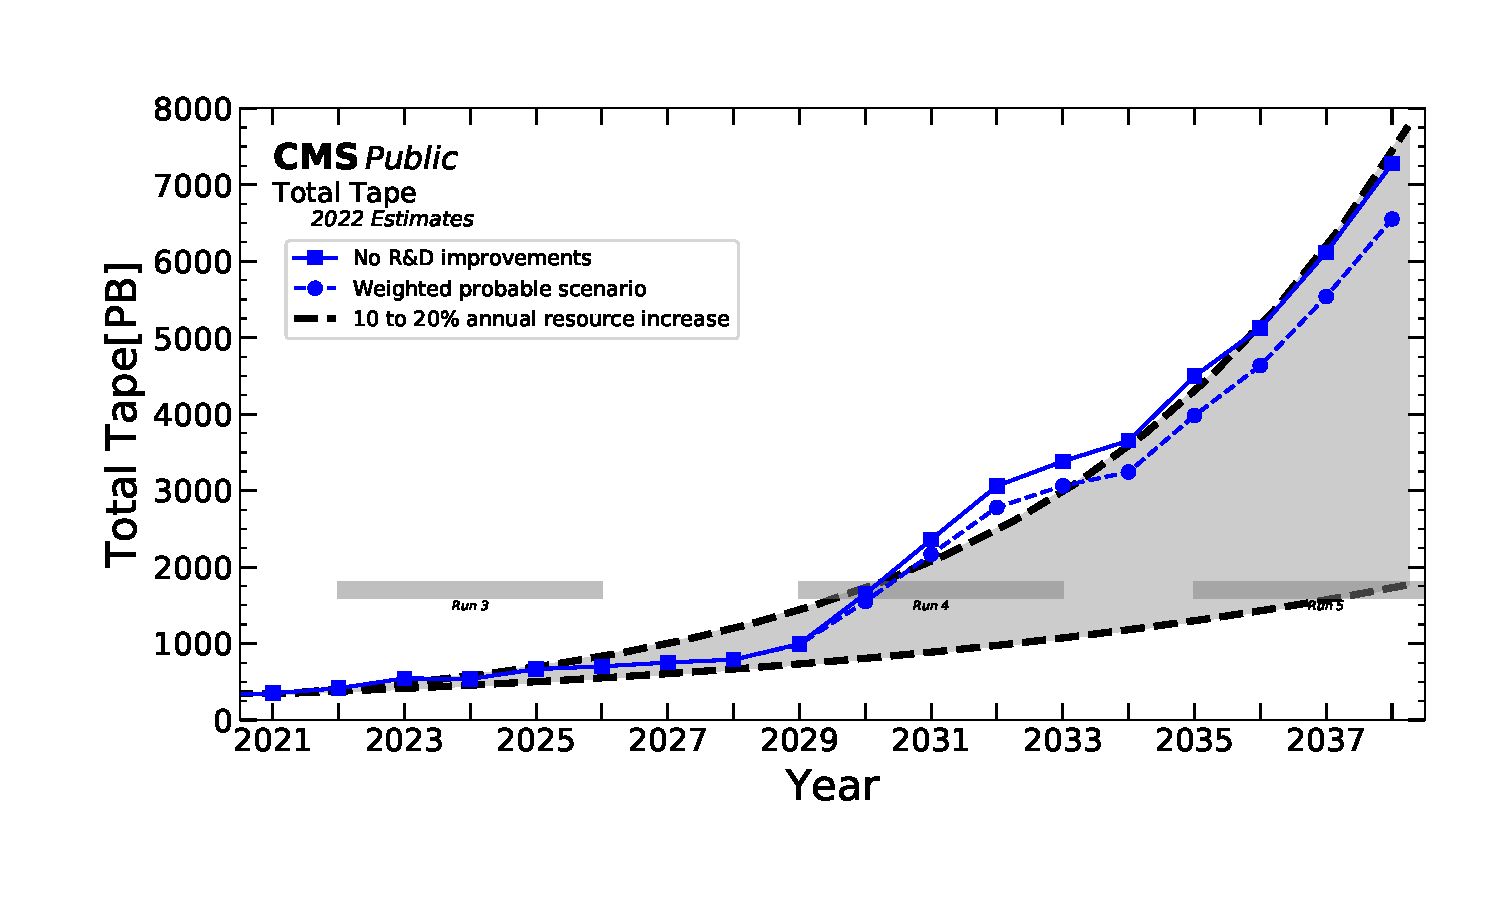
\includegraphics[width=.9\textwidth]{fig/cyber/tape_cms2022.pdf}
    \caption[HL-LHC tape usage projections at CMS]{
        The HL-LHC tape usage projections at CMS as a function of time, showing data production rates of over 0.5 EB per year after 2030~\cite{CMSComputingReport2022}.
    }
    \label{fig:tape_projections}
\end{figure}

With many PB, soon to be EB, of data that needs to be distributed all over the world, National Research and Education Networks (NRENs) are critical to the continued operation of CMS, and the LHC in general. 
However, NRENs are entirely opaque to their users---that is, users have no control over the share of the network that they receive---resulting in highly variable networking performance. 
This kind of unmanaged networking is referred to as ``best effort'' service, and it already presents significant challenges to CMS operators running production data transfers. 
For example, high priority data transfers will unpredictably slow down, or even fail, making any precise coordination impossible. 
These kinds of issues are furthermore difficult to diagnose: with an opaque network, operators must coordinate between the data storage site administrators and network engineers just to gain a preliminary understanding of where the problem may lie. 
An increase in data volumes by an order of magnitude would inflate these challenges into significant barriers for the data operation at CMS, and the LHC in general. 
Thus, a novel solution is imperative in order to guarantee the success of the HL-LHC~\cite{HEPSoftwareFoundation2017, Zurawski2021}. 

\section{Software defined networking}
If CMS operators could have a specified bandwidth reserved for a high-priority, production data transfers could be achieved on a more well-defined timescale. 
Meanwhile, lower priority data transfers, including user traffic, could share the unreserved bandwidth as they do today. 
This functionality is exactly provided by software defined networking (SDN)~\cite{SDNSurvey}, which enables the allocation of networking resources in the same way that CPUs and memory are allocated on shared computing clusters. 
With this model, CMS operators could hold the network accountable for the ``promises'' (bandwidth guarantees) it has made. 
By comparing data movement speed against the network promise and storage site diagnostics, which are already maintained, CMS operators could easily determine, and therefore more quickly address, bottlenecks in throughput. 
Therefore, by incorporating SDN into the existing data movement infrastructure, CMS would be able to efficiently and reliably move EB of data around the world. 
Furthermore, while described in the context of CMS, SDN could be used to address the data movement requirements for other LHC experiments like ATLAS, or even other large-scale science experiments. 

\section{Rucio}
The distribution of CMS data is managed through Rucio, an open-source data management framework designed specifically for large-scale science~\cite{Rucio2019}. 
In practice, CMS operators define ``rules'' which represent the replication of one or more datasets one or more data storage sites. 
The operator also assigns a priority to each rule that can be changed at any time. 
Until the replication is complete, the requisite data transfers are organized for each rule. 
These data transfers are initialized and managed by the File Transfer Service (FTS)~\cite{FTS3}, starting with the transfers belonging to the highest priority rule. 

\section{SENSE}
The Energy Sciences Network (ESNet), the NREN used by the CMS and ATLAS collaborations in the United States, has developed an SDN product called SENSE: SDN for end-to-end networked science at the exascale~\cite{SENSE}. 
It is designed to provide users with enhanced interactivity via an ``intent-based'' interface, allowing for the precise management of network resources---the exact functionality needed for HL-LHC data movement. 
SENSE provides this interactivity through a novel configuration of the data storage sites (Fig.~\ref{fig:sense_site}) that allows data to be accessed across many different IPv6 subnets simultaneously. 
These subnets logically divide the network traffic which, in turn, enables SENSE to allocate bandwidth. 

\begin{figure}[htb]
    \centering
    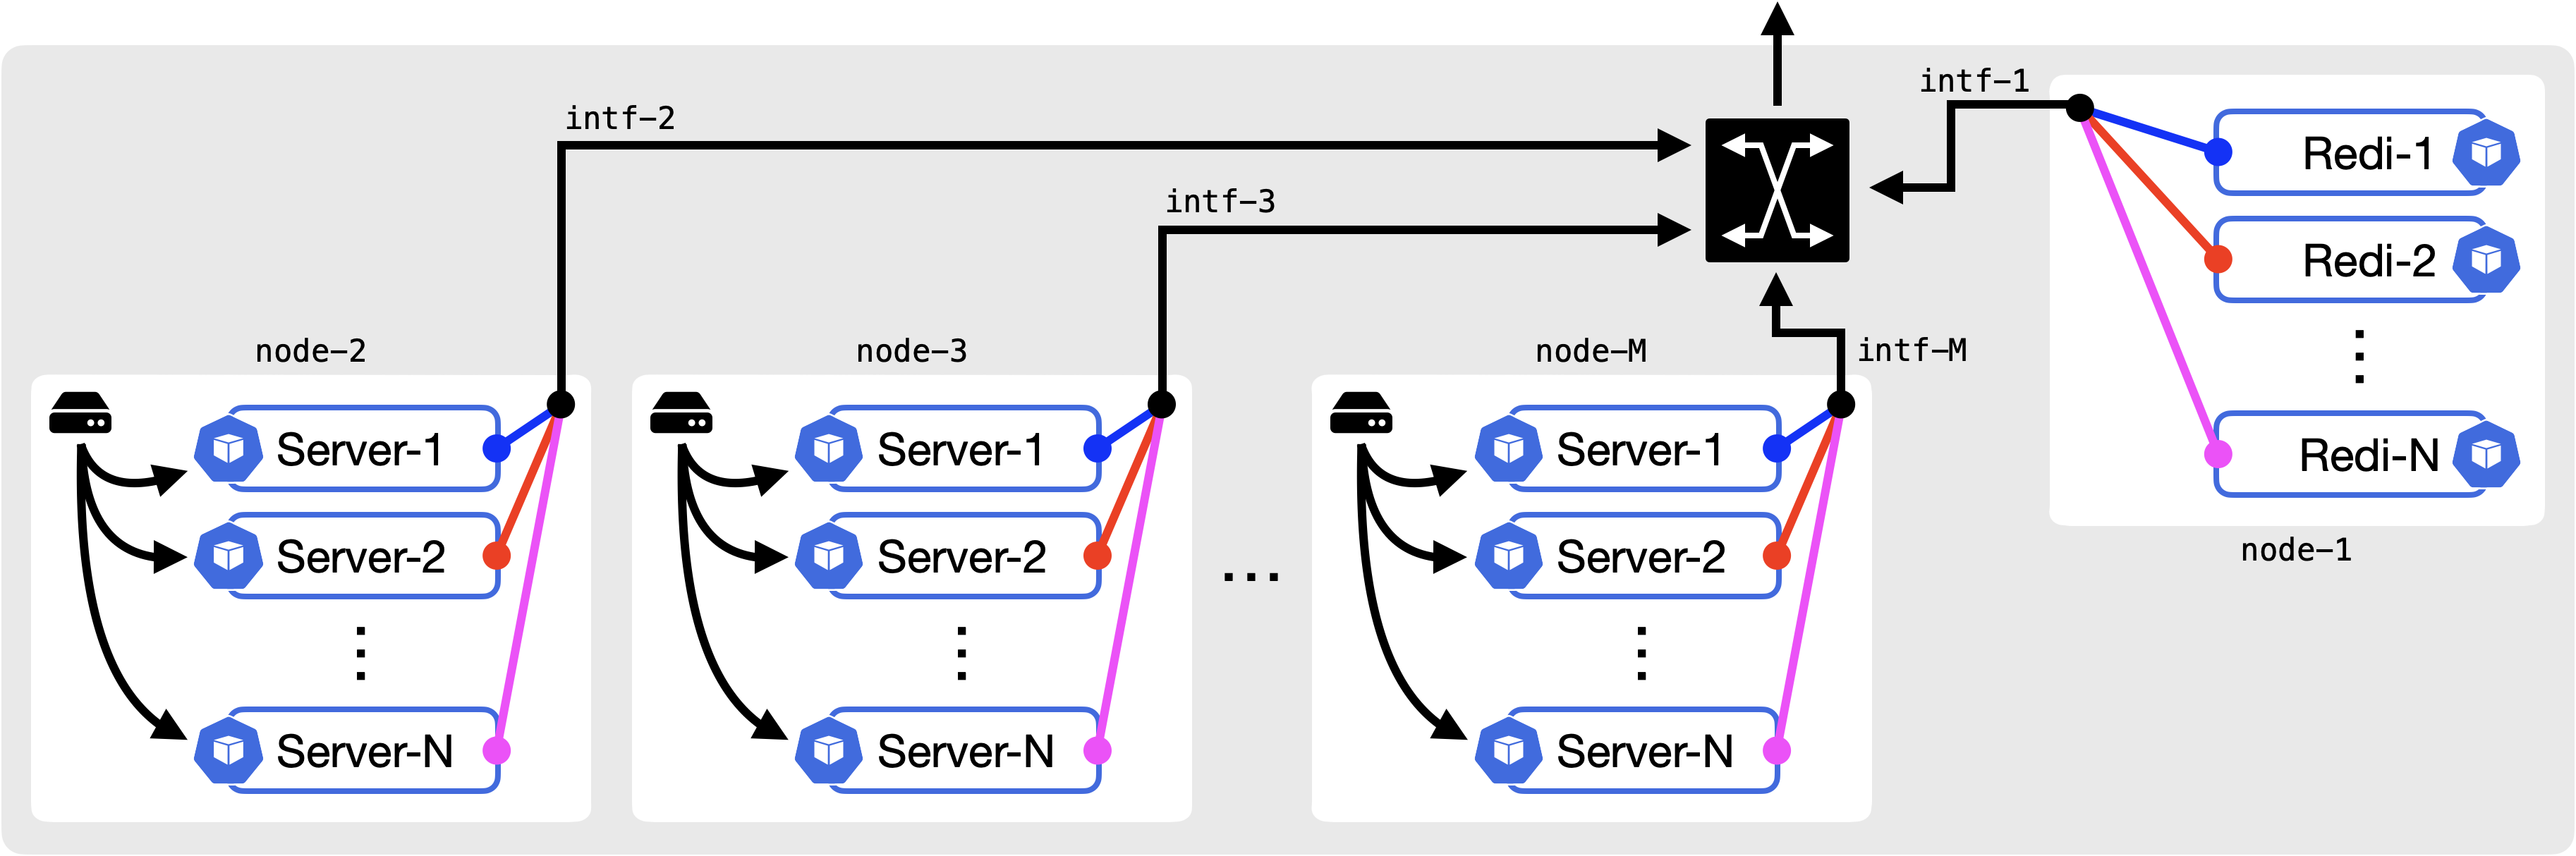
\includegraphics[width=.9\textwidth]{fig/cyber/rucio-sense_site.png}
    \caption[Rucio-SENSE site configuration]{
        A generic site configuration that enables SENSE capabilities, where each ``redirector'' services a different bandwidth allocation by directing traffic for that allocation to one of the data servers connected to it. 
        Each data server has equal access to the underlying filesystem.
    }
    \label{fig:sense_site}
\end{figure}

\section{Rucio-SENSE interoperation model}
In order to leverage SENSE for CMS data distribution, the close interoperation of Rucio and SENSE must be implemented with little-to-no changes to Rucio, as it is already used in production. 
Specifically, priorities assigned to each rule in Rucio should correspond to an appropriate bandwidth reservation made through SENSE, and changes to that rule should result in changes to the reservation. 
We designed and implemented a Data Movement Manager (DMM) to perform this crucial translation. 
Importantly, DMM also holds the intelligence for determining what an ``appropriate'' bandwidth reservation is for a given priority. 
DMM is therefore the keystone of the Rucio-SENSE interoperation model (Fig.~\ref{fig:rucio_sense_basic}) first described in Ref.~\cite{Guiang:2022tgi}:
\begin{enumerate}
    \item A Rucio operator initializes a rule with some priority which requests one or more dataset transfers, where each transfer may involve a different pair (source and destination) of sites
    \item Rucio sends the following data to DMM for each transfer:
    \begin{itemize}
        \item Total transfer size
        \item Source site
        \item Destination site
        \item Priority
    \end{itemize}
    \item DMM processes the data from Rucio:
    \begin{enumerate}
        \item If the transfer has no priority, place it on best effort service (skip steps below)
        \item Reserve an IPv6 address at the source and destination site
        \item Compute the bandwidth provision (i.e. promise) appropriate for the transfer priority
    \end{enumerate}
    \item DMM requests a new promise from SENSE that implements the provisioning from (3c), reprovisioning existing promises where appropriate
    \item DMM sends the IPv6 addresses it reserved to Rucio
    \item Rucio injects the IPv6 addresses into the FTS request
    \item SENSE takes one of the following actions:
    \begin{enumerate}
        \item Begin the construction of a new guaranteed-bandwidth link
        \item Do nothing; the transfer will be provided best effort service
    \end{enumerate}
    \item SENSE sends identifying metadata for the link back to DMM
\end{enumerate}
Several of these steps offer the opportunity for further optimization. % TODO: rephrase this section
In particular, it is clear that a future implementation may see the integration of DMM into Rucio such that the operations in steps (2) through (5) can be implemented to better handle a large number of transfers.
Before then, however, DMM provides an isolated testbed in which the fundamental design of the interoperation model can be prototyped.
Step (3c) is of particular interest, because it implements the bandwidth provisioning--the central deliverable of this work.
The provisioning decision could be designed, for example, to allow Rucio operators to schedule transfers: e.g. \textit{move Dataset A to Site B in one week}.
Alternatively, the decision could pack the maximum available bandwidth between two sites as a function of each transfer's priority.
In any case, this interoperation model provides a flexible testbed for evaluating these ideas and producing concrete metrics on their scalability, practicality, and efficiency.

\begin{figure}[htb]
    \centering
    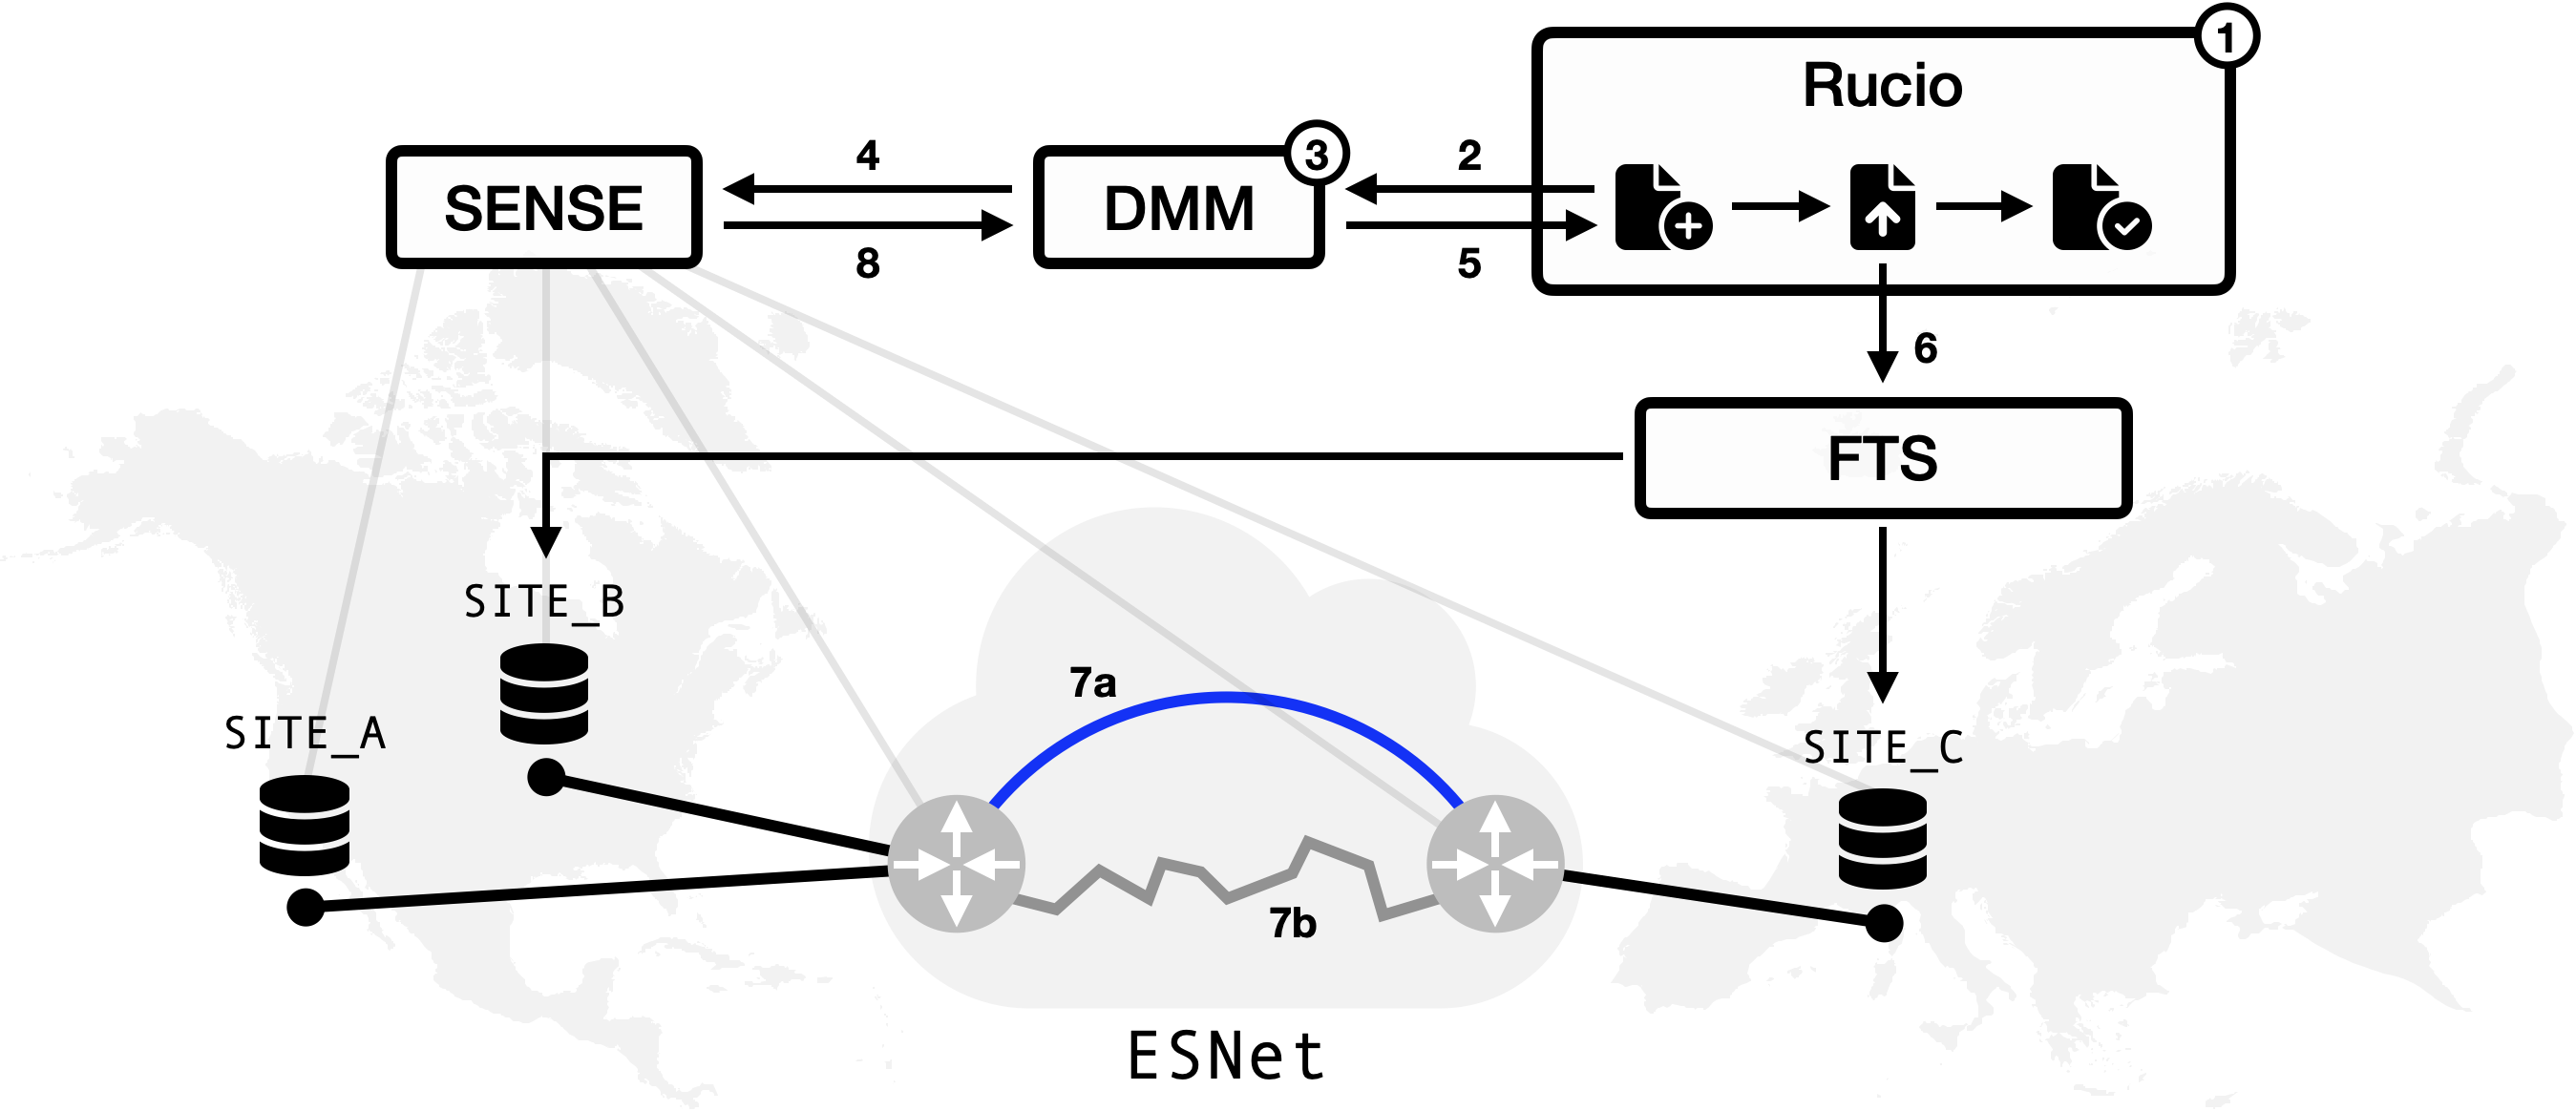
\includegraphics[width=.9\textwidth]{fig/cyber/rucio-sense_basic.png}
    \caption[Rucio-SENSE interoperation workflow]{
        A simplified diagram of the Rucio-SENSE interoperation workflow, taken from Ref.~\cite{Guiang:2022tgi}, with numbered steps: 
        (1) a rule is initialized; 
        (2) Rucio sends transfer description to DMM; 
        (3) DMM translates Rucio request into SENSE provision; 
        (4) DMM sends provision request to SENSE; 
        (5) DMM sends a source IPv6 and destination IPv6 to Rucio;
        (6) Rucio injects IPv6s from previous step into the FTS request;
        (7) Either (a) SENSE builds dedicated service or (b) default to best effort service; 
        (8) SENSE sends service metadata to DMM.
    }
    \label{fig:rucio_sense_basic}
\end{figure}

\section{Demonstrations}
The Rucio-SENSE interoperation was first demonstrated in a simple test involving two sites, one at UCSD and another at Caltech. 
These institutions were selected because they each maintain highly active ``\Tier{2}'' computing facilities, which are the endpoints of real CMS production data transfers. 
In order to simulate this kind of network traffic, the IPerf tool was used to emulate activity across best effort network services. 
At the same time, a private instance of Rucio was deployed with only UCSD and Caltech as known sites. 
After the best effort network traffic saturated the 10 Gb/s network link between the two sites, we initialized a rule in Rucio that requested a replica of 750 GB of data stored at UCSD to be made at Caltech. 
This rule was assigned a high priority. 
Once the rule was initialized, DMM requested bandwidth reservation of 7 Gb/s for the data transfers. 
Importantly, the bandwidth received may never fall below a SENSE bandwidth reservation, but it is allowed to exceed it. 
As shown in Fig.~\ref{fig:rucio_sense_demo}, the priority data transfers were completed in a timely manner thanks to the large amount of bandwidth reserved for them. 
The throughput for best effort traffic, meanwhile, was suppressed until the priority transfers finished. 
This test shows the fundamental action of the Rucio-SENSE interoperation model from end to end, demonstrating that the two technologies could successfully work in concert. 
Though simple, the test was the result of many months of work, as many aspects of the implementation of this model are novel, and therefore non-trivial. 

A more complicated test was recently performed involving a testbed site at Fermilab (FNAL) in addition to the existing Caltech and UCSD sites. 
In this test, high-priority data transfers are started between UCSD and Caltech---in particular, they are assigned a priority of 5. 
Then, data transfers between FNAL and Caltech are initiated with a middling priority of 3. 
Finally, we began another set of data transfers between UCSD and Caltech with a low priority of 2. 
All sites had 100 Gb/s connectivity between each other, so the priorities correspond to 50 Gb/s, 30 Gb/s, and 2 Gb/s, respectively---there was no best-effort traffic in this test. 
As the data moved from source to destination, we swapped the priority assignments every one to two hours. 
In Fig.~\ref{fig:rucio_sense_demo_big}, it can be seen that the bandwidth is appropriately limited for the three data transfers at any one time. 

\begin{figure}[htb]
    \centering
    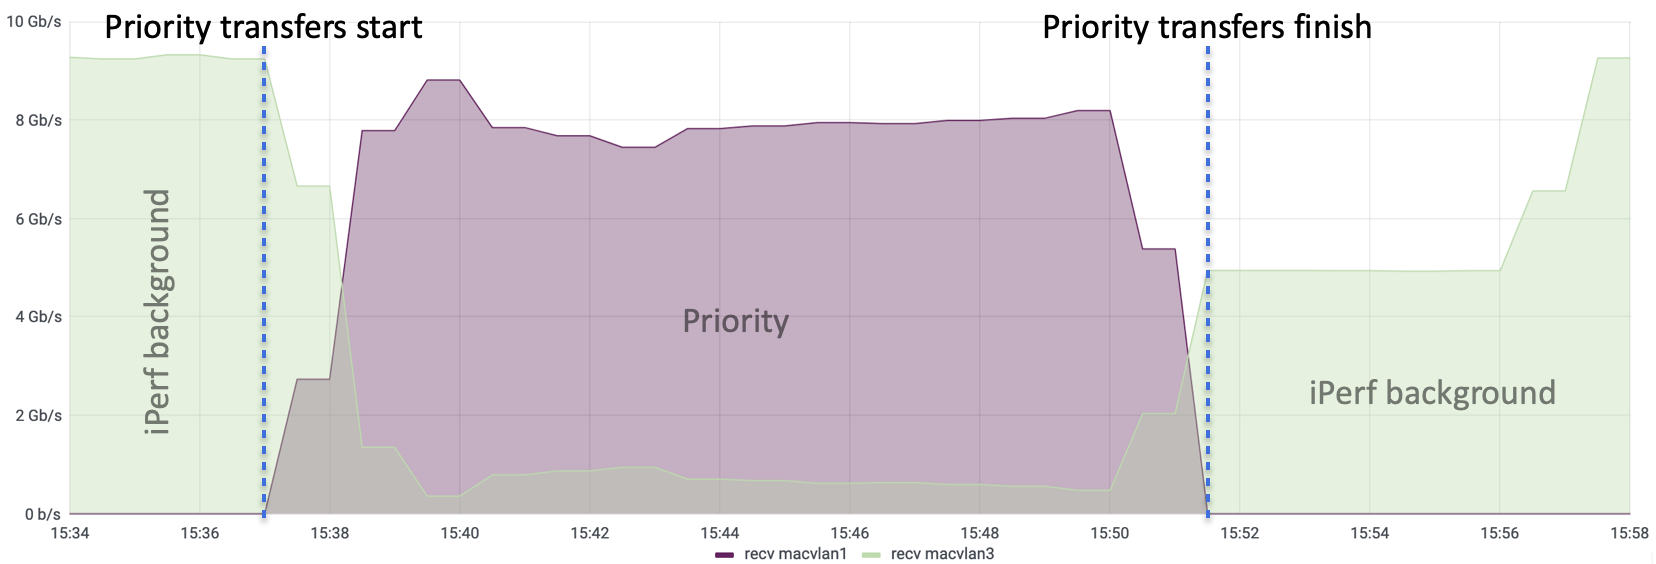
\includegraphics[width=.9\textwidth]{fig/cyber/rucio-sense_demo.png}
    \caption[Rucio-SENSE interoperation throughput with 2 sites in the testbed]{
        Throughput measurements of the first demonstration of the Rucio-SENSE interoperation prototype involving three sites: UCSD and Caltech. 
        Background traffic is simulated with the IPerf tool, emulating activity across best effort network services. 
        Then, a set of priority data transfers are initialized between the two sites with at least 7 Gb/s of requested bandwidth. 
        This throttles the best effort traffic until the priority transfers are complete and the reservation is released. 
    }
    \label{fig:rucio_sense_demo}
\end{figure}

\begin{figure}[htb]
    \centering
    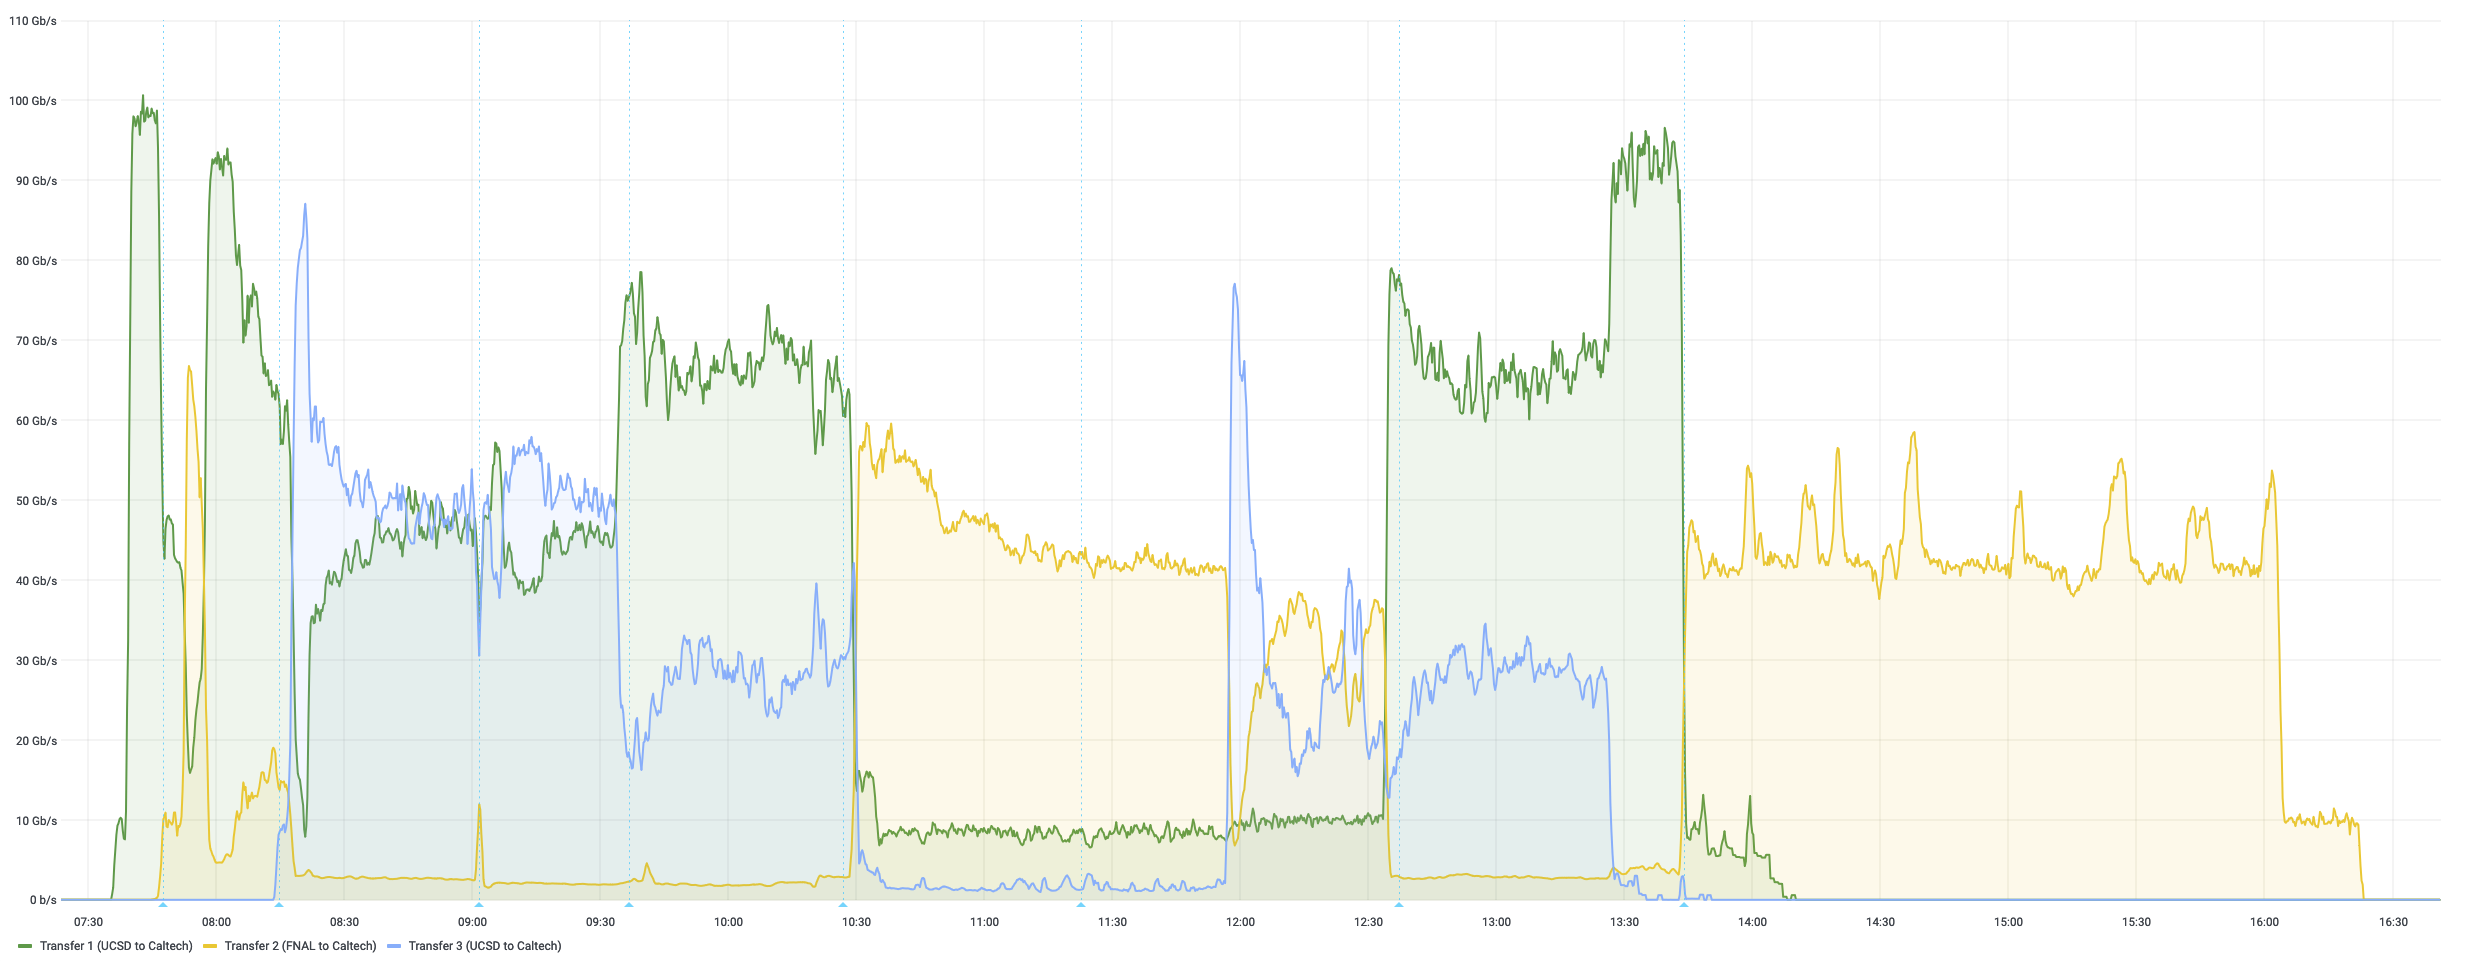
\includegraphics[width=.9\textwidth]{fig/cyber/rucio-sense_demo_big.png}
    \caption[Rucio-SENSE interoperation throughput with 3 sites in the testbed]{
        Throughput measurements of a demonstration of the Rucio-SENSE interoperation prototype involving three sites: UCSD, FNAL, and Caltech. 
        Three sets of data transfers are started simultaneously: one from UCSD to Caltech with priority 5, another from FNAL to Caltech with priority 3, and one more from UCSD to Caltech with a priority of 2. 
        Every one to two hours, the priorities are swapped between the three. 
        The throughput for each transfer correctly reflects the appropriate bandwidth for its priority at any one time. 
        In particular, the priorities 5, 3, and 2 correspond to 50 Gb/s, 30 Gb/s, and 20 Gb/s, respectively.
      }
    \label{fig:rucio_sense_demo_big}
\end{figure}

\section{Next steps}
With the Rucio-SENSE interoperation model now demonstrated successfully multiple times, we are now interested in including more sites in the existing testbed as we walk the project closer to production. 
In addition, the intelligence of the DMM priority allocation will continue to be refined, with special attention given to the possibility of data transfer scheduling. 

\section{Acknowledgements}
This chapter is a partial reproduction of the paper ``Integrating End-to-End Exascale SDN into the LHC Data Distribution Cyberinfrastructure'', in the proceedings of PEARC 2023 (doi:10.1145/3491418.3535134). 
This ongoing work is partially supported by the US National Science Foundation (NSF) Grants OAC-2030508, OAC-1841530, OAC-1836650, MPS-1148698, and PHY-1624356.
In addition, the development of SENSE is supported by the US Department of Energy (DOE) Grants DE-SC0015527, DE-SC0015528, DE-SC0016585, and FP-00002494.
